\subsection{Failure analysis}
\label{sec:failure}

\begin{figure*}[t]
\centering
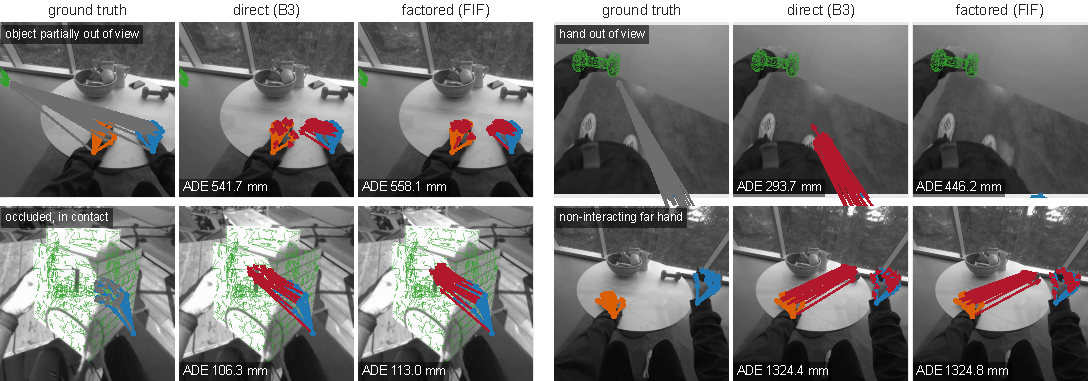
\includegraphics[width=\textwidth]{../figures/fig5_failure.pdf}
\caption{Failure cases: the worst fold-A frame of the factored model in four categories of difficulty, with the direct model on the same frame. Ground-truth vectors are grey, predictions red; the crop is chosen to contain the true endpoints and light grey marks regions outside the image, so a skeleton drawn there is a hand that the camera does not see. Top left: the object (green, left edge) is almost out of the image and the hands are far from it. Top right: the right hand is below the image; the direct model still anchors its vectors, the factored model does not. Bottom left: the hand grips the birdhouse and most of its joints are hidden behind the object; both models err by more than 100\,mm on a hand whose true field has a median magnitude below 15\,mm. Bottom right: the right hand rests on a mouse while the left rests 1.3\,m away; the true field of the left hand is a 1.3\,m vector that no model predicts.}
\label{fig:fail}
\end{figure*}

\Cref{fig:fail} shows the worst held-out frame of the factored model in each of four categories, and the category statistics explain where the mean of \cref{tab:main} is decided. We group the 5,955 fold-A validation frames by properties of the ground truth, computed once and applied to both models.

\paragraph{Non-interacting hands dominate the tail}
In 1,152 frames (19\% of the validation set) at least one hand has a median field magnitude above 200\,mm: the hand is not interacting with the object at all, and the label is the vector to an object the person is holding in the other hand, has put down, or is about to pick up. On these frames the factored model averages 102\,mm and the direct model 105\,mm. The 32 frames in which the object is essentially out of the reference image average 426 and 429\,mm. The single worst frames are all of one kind: subject XYZ109 types or waves with one hand while the mouse rests far away, and the true field is a vector of more than one metre that both models miss by the same amount (\cref{fig:fail}, bottom right). Such frames are legitimate under the task definition but carry no information about hand-object interaction; whether they should count towards an interaction-field metric is a question for the benchmark rather than for the models.

\paragraph{One unseen object accounts for a sixth of the error}
The mouse is handled by a single subject in the training release, and that subject (XYZ109) is held out in fold A, so the fold-A validation set tests the mouse as an unseen object with 11,130 joint targets at 134.5\,mm (direct: 136.3\,mm). Its contribution to the mean, the product of its share of joints and its stratum error, is 7.1\,mm of the factored model's 44.4\,mm; the dumbbell, whose exercise sequences move the free hand far from the weight, contributes a further 10.9\,mm at 65.1\,mm over 35,427 joints. Two of nine objects therefore account for 18 of the 44\,mm. The remaining seven objects lie between 24.5\,mm (vase) and 50.2\,mm (orange juice), and the factored model improves on the direct one for all but two of them (orange juice by 3.7\,mm and dinotoy by 0.1\,mm in the wrong direction, birdhousetoy by 5.3\,mm in the right one); on the two heavy contributors it gains as well, 2.8\,mm on the dumbbell and 1.8\,mm on the mouse. On fold B, where the held-out subjects handle twelve objects that all appear in training, the object errors range from 19.4 to 51.4\,mm and the factored model improves on ten of the twelve.

\paragraph{Occlusion by the object is not where the gain is}
The 3.0\,mm gain on the \emph{occluded-or-outside} stratum of \cref{tab:strata} might suggest that the geometric route helps when fingers are hidden behind the object. It does not. Take the 812 frames in which a hand is inside the image but more than half of its joints are occluded by the posed mesh and its median field magnitude is below 15\,mm, that is, the hand is wrapped around the object. On those frames both models score 29\,mm (factored 29.3, direct 29.2). The stratum gain comes from the joints \emph{outside} the image, where the factored model is 21\,mm better. For joints within 15\,mm of the object, moreover, both models are barely better than predicting the zero vector (14.0 and 14.6\,mm against a bound of 15\,mm): at contact the models have learned that the field is small but not which small vector it is, and the object's own annotation noise of 1.5 to 3.5\,mm~\cite{rim2026show3d} is a floor on what can be recovered there.

\paragraph{Hands outside the image}
When a hand is below 10\% inside the reference image (311 frames), the factored model averages 152\,mm and the direct model 165\,mm. Because the hand is not observed, both models extrapolate from the other hand, the object and the body; the factored model's advantage of 21\,mm on this stratum is the largest of any and is consistent across folds and views (\cref{fig:strata}c). The worst individual frame in this category (\cref{fig:fail}, top right) is one where the direct model still anchors its vectors to the invisible hand and the factored model does not, so the gain on the stratum is a property of the average, not of every frame.

\paragraph{Clean frames}
On the 896 frames in which the object is in view, both hands are inside the image, at least 80\% of joints are visible and the median field magnitude lies between 15 and 60\,mm, the factored model scores 30.4\,mm and the direct model 32.7\,mm. The difference on these frames (2.3\,mm) is larger than the overall difference (1.7\,mm) in absolute terms and much larger in relative terms (7\%), which is the cleanest statement of what geometric supervision buys when the scene is well observed.
